% !TEX root = ./Basilisk-inertialUKF-20190402.tex

\newpage

\section{Test Description and Success Criteria}

This filter builds on the long test suite of other SRuKFs in Basilisk. This test focuses on the differences from other filters: the measurement update. 
In order to keep a rigorous process, the state propagation is test once more as well.

\subsection{Test 1: Individual Methods Tests}

The first test in this suite runs methods individually:

\begin{itemize}
\item{pixel Line uKF Meas Model:} This test creates a Sigma Point matrix and predicts the measurements model's computations. It compares the expected output and the actual output down to 1E-15 
\item{pixel Line State Prop:} This test runs the state propagation after one step of simulation. It's main goal is to test the RK4, as it runs one in python and compares them down to 1E-15
\end{itemize}


\subsection{Test 2: State Propagation}

This test runs a pure propagation test. The states are set to a fixed value and integrated with the filter.
This shows filter stability in the simple case and a very low tolerance for error is permitted (1E-10). 

Input circle measurement parameters are:
\begin{itemize}
    \item Input circlesCenters = [100, 200]
    \item Input circlesRadii = [100]
    \item Input planetIds = [2]
    \item Input cirlcesInMsg = msg
    \item Input planetId = 2
    \item Input countHalfSPs = 9
    \item Input numStates =9
\end{itemize}

Input attitude parameters are:
\begin{itemize}
\item Input sigma\_BN = [0, 0.2,-0.1]
\item Input omega\_BN\_B = [0.,0.,0.]
\end{itemize}

\begin{itemize}
    \item Input sigma\_CB = [-0.2, 0., 0.3]
    \item Input focalLength = 1
    \item Input sensorSize = [10,10]
    \item Input resolution = [512, 512]
\end{itemize}

Figures \ref{fig:EnergyProp} and \ref{fig:StatesPlotProp} show the results for the energy and state errors. 
 \begin{figure}[htbp]\centerline{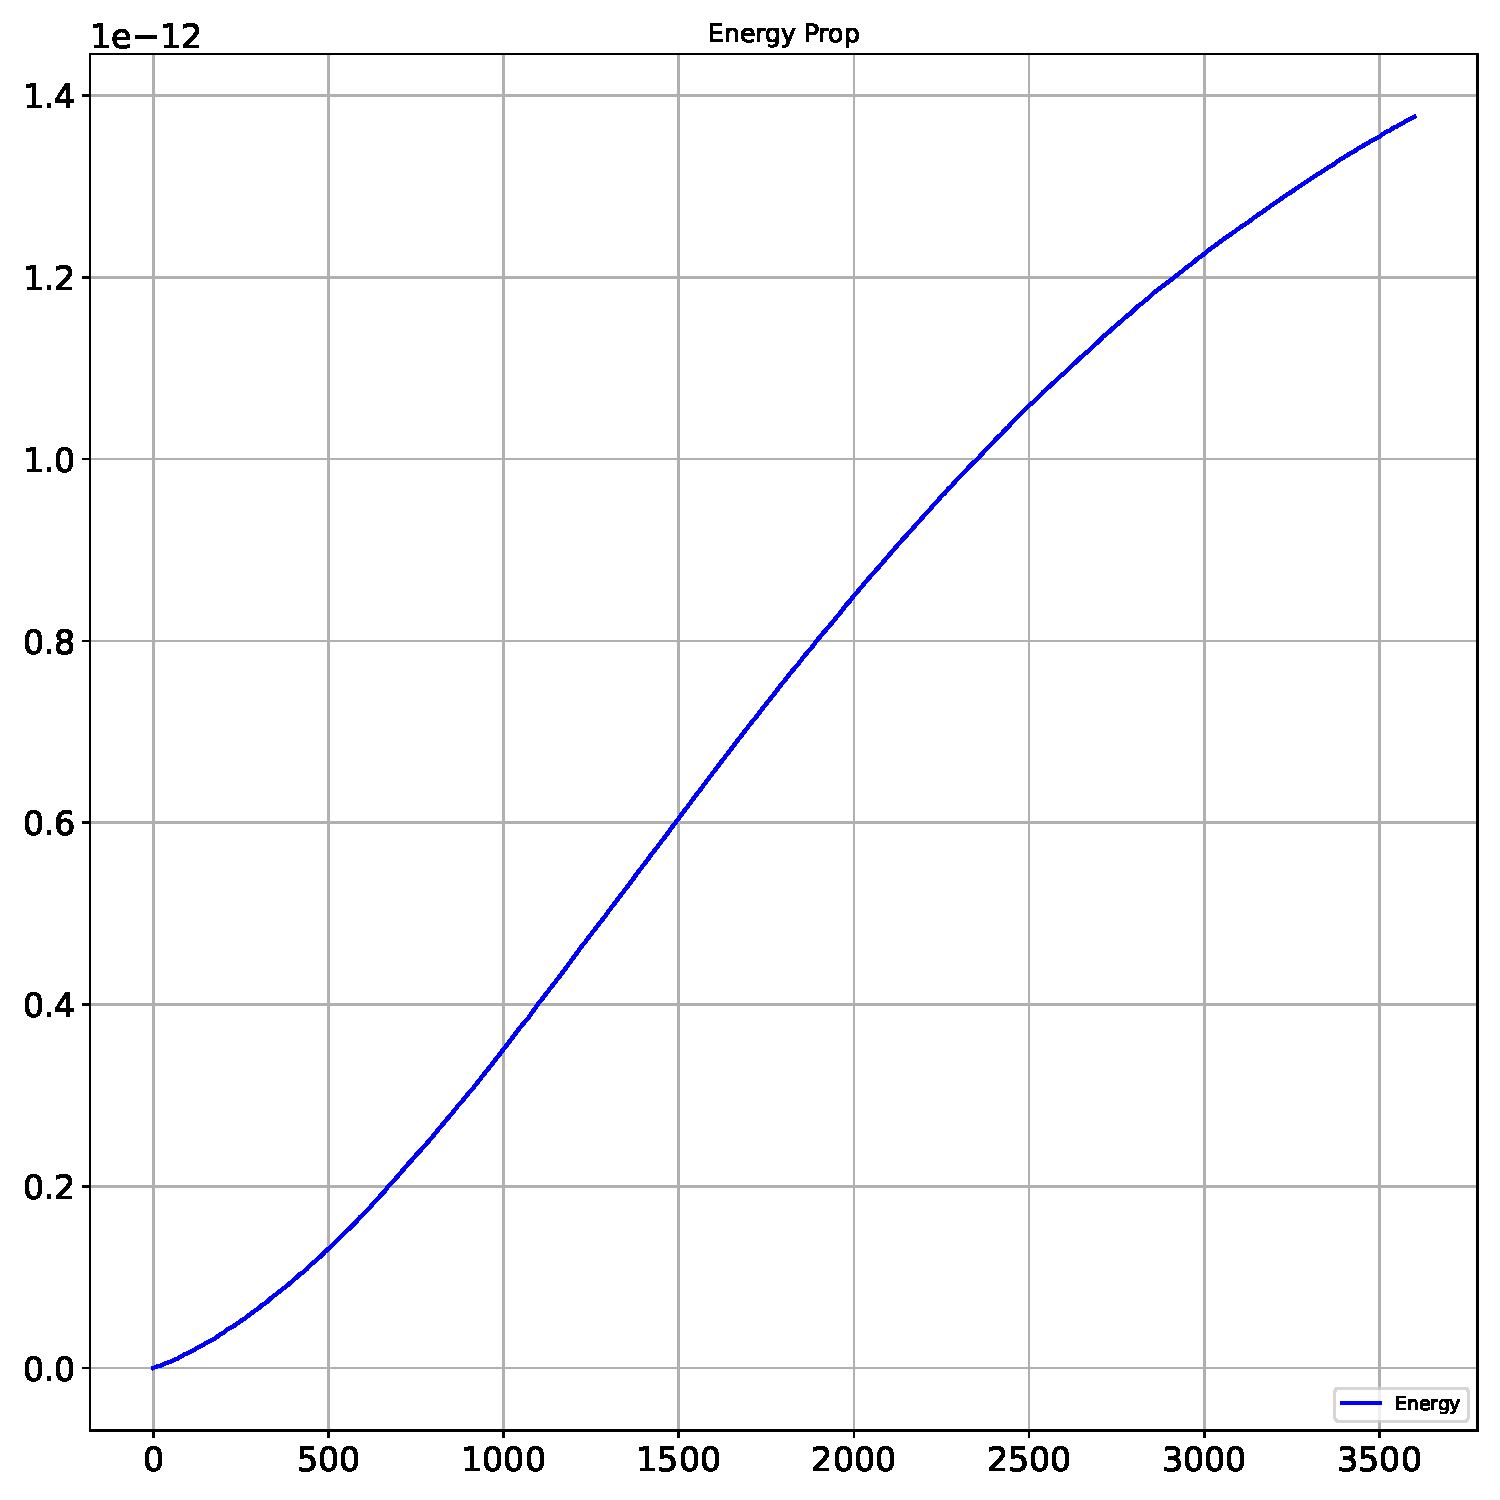
\includegraphics[height=0.9\textwidth, keepaspectratio]{AutoTeX/EnergyProp}}\caption{Orbital Energy}\label{fig:EnergyProp}\end{figure}
 \begin{figure}[htbp]\centerline{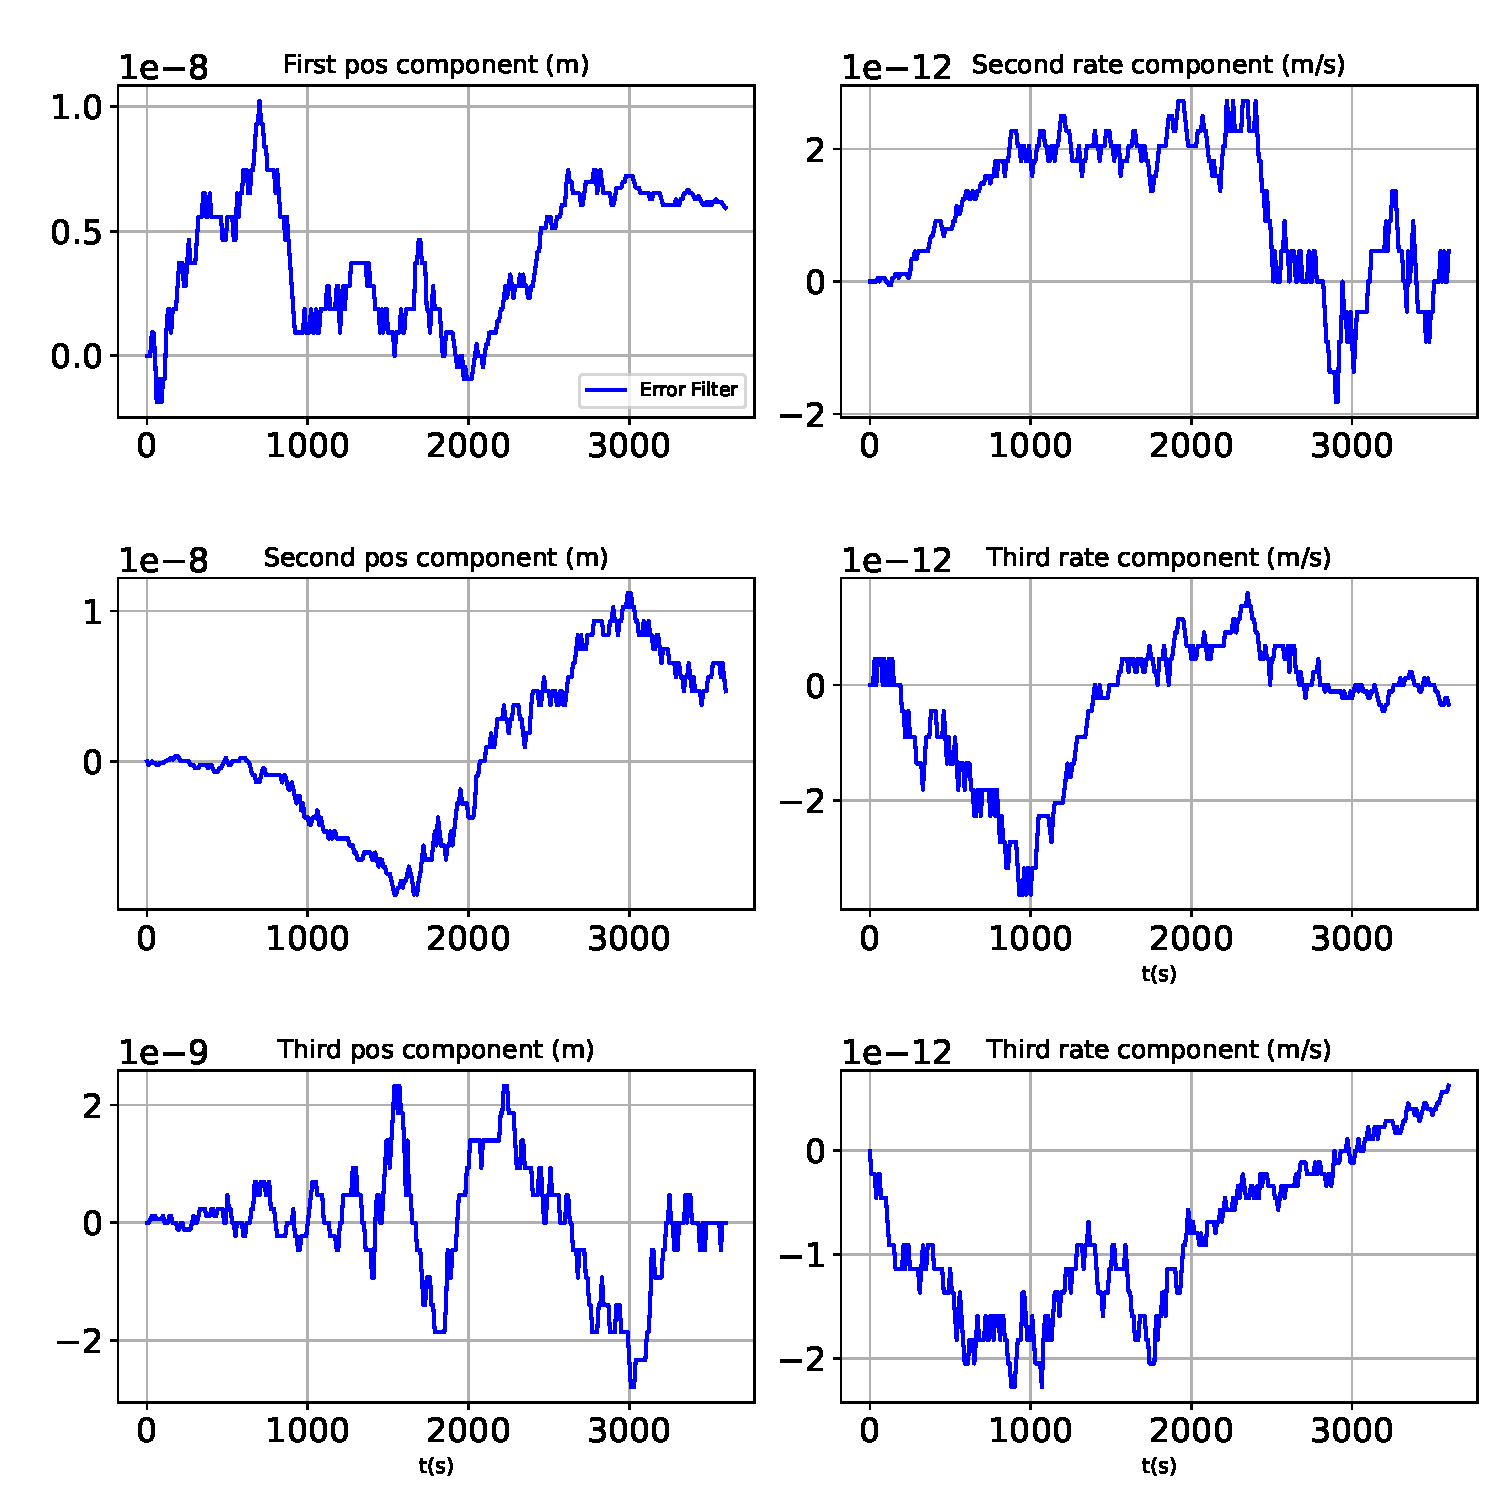
\includegraphics[height=0.9\textwidth, keepaspectratio]{AutoTeX/StatesPlotProp}}\caption{State error}\label{fig:StatesPlotProp}\end{figure}
 
Energy is conserved, and state errors are down to machine precision
  
\section{Test Parameters}

\begin{table}[ht]
\centering
\begin{tabular}{c|c}
\hline
\hline
\textbf{Output Value Tested}     & \textbf{Tolerated Error}  \\ \hline
Test 1-Measurement 	       & 1E-15      		             \\
Test 1-Propagation	               & 1E-15     	                  \\
Test 2-Energy  	                       & 1E-10    		                   \\
Test 2-States  	                       & 1E-10    		                   \\
\end{tabular}
\end{table}

\section{Test Results}

\begin{table}[H]
	\caption{Test results}
	\label{tab:results}
	\centering \fontsize{10}{10}\selectfont
	\begin{tabular}{c | c}
		\hline\hline
		\textbf{Check} 			&\textbf{Pass/Fail} \\ 
		\hline
	   Test 1	   			& PASS \\ 
	   Test 2	   			&PASS \\ 
	   \hline\hline
	\end{tabular}
\end{table}
